\subsection{GUI}\label{subsec:gui}
Die Funktionen welche von Terasic für die Gestaltung des GUI zur Verfügung gestellt werden sind für unser Projekt zu ineffizient. Um ein Text anzuzeigen verwendet Terasic eine Funktion die ein Alpha Blending durchführt. Dieses wird immer an den Rändern der Buchstaben durchgeführt. Dabei wird die Schriftfarbe mit der Hintergrundfarbe gemischt. Dieser Prozess nimmt viel Zeit in Anspruch. Wodurch bei jedem neuen zeichnen eines Texte Strings zugeschaut werden kann wie die Pixel gezeichnet werden. Dies ist für unser Projekt unbrauchbar. Zudem hat uns die von Terasic verwendete Schriftart nicht gefallen. Daher entschieden wir uns eine eigene Funktion zu schreiben welche Text stringe zeichnet. Diese ist im Modul  \textbf{simple\_text.c} realisiert.

\paragraph{simple\_text.c}\mbox{}\\
\begin{figure}[h]
	\centering
	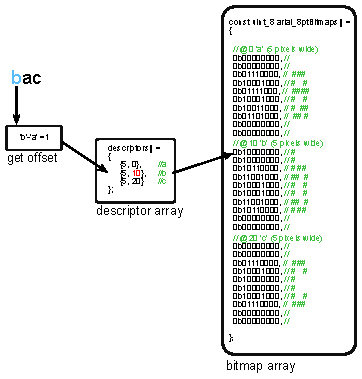
\includegraphics[width=0.8\textwidth]{the_dot_factory.pdf}
	\caption{Bitmap und Discriptor Array.}
	\label{img:bitmap}
\end{figure}
Da das LCD nur in der Lage ist Pixel zu setzen gestaltet sich das zeichnen einer Schrift eher mühsam. Mit dem open source tool "The Dot Factory" generierten wir uns eine Bitmap für die Schrifftart Arial welche 22points gross gewählt ist. Das tool generiert zwei Arrays. Im Character Bitmap Array sind die Character in einer Bitmap gespeichert. Das Character Descriptor Array enthält Informationen über die Breite jedes Characters und den Offset in der Character Bitmap. Um den Ort eines Characters zu bestimmen wird der Character minus des ersten Character in der Bitmap gerechnet.  Dies ergibt den Index für das Descriptor Array in welchem der Offset für die Bitmap gespeichert ist. In Abbildung \ref{img:bitmap} ist dieser Prozess veranschaulicht. In diesem Beispiel besteht die Bitmap aus den Buchstaben abc. Für den Buchstaben b wird der Offset 1 ausgerechnet. Im Descriptor Arrey ist auf Position 1 die Breite 5 gespeichert und der Offset 10 für die Bitmap. Mit diesen Informationen kann die Funktion \textit{print\_string(x,y,color,font,font\_descriptor,string)} einen Text String zeichnen. Dabei werden nur die Pixel gezeichnet welche in der Bitmap auf 1 gesetzt sind.


\paragraph{gui.c} \mbox{}\\
In diesem Modul sind mit der Funktion \textit{print\_string(x,y,color,font,font\_descriptor,string)} aus dem Modul  \textit{simple\_text.c} und der Funktion \textit{LCD\_DrawRect(xs,ys,xe,ye,color)} aus dem Modul \textit{LT24\_controller.c} die einzelnen Menüs dargestellt. 